\section*{Conics\ \normalfont\scriptsize{$(\varepsilon,a,b,c,h,k,p,\ell\in\mathbb{R})$, $\varepsilon\equiv$ eccentricity, $c\equiv$ focal distance, $p \equiv$ focal parameter, $\ell \equiv$ semi-latus rectum, $a\equiv$ semi-major axis, $b \equiv$ semi-minor axis, $\ell = p \varepsilon$, $c=a\varepsilon$}, $p+c =a/\varepsilon $, $(h,k)\equiv$ center, $(h,k)_{\text{parabola}}\equiv$ vertex }
\begin{align*}
&\text{Vertical parabola: }(y\!-\!k)\!=\!\frac{1}{4p}(x\!-\!h)^2,\;\varepsilon\!=\!1 \;\;\text{Circle: }(x\!-\!h)^2\!+\!(y\!-\!k)^2\!=\!a^2,\;\varepsilon\!=\!0 \\
&\text{Ellipse: }\frac{(x\!-\!h)^2}{a^2}\!+\!\frac{(y\!-\!k)^2}{b^2}\!=\!1,\;\varepsilon\!=\!\sqrt{1\!-\!\left(\frac{b}{a}\right)^2}\; \hspace{1cm}
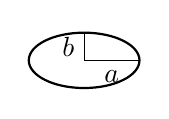
\begin{tikzpicture}[baseline={(0,-1pt)}]
  \draw[thick] (0,0) ellipse (20pt and 10pt);
  \draw (0,0) -- (20pt,0) node[midway,below] {$a$};
  \draw (0,0) -- (0,10pt) node[midway,left] {$b$};
\end{tikzpicture} \\
&\text{Hyperbola: }\frac{(x\!-\!h)^2}{a^2}\!-\!\frac{(y\!-\!k)^2}{b^2}\!=\!1,\;\varepsilon\!=\!\sqrt{1\!+\!\left(\frac{b}{a}\right)^2}\; \hspace{10pt}
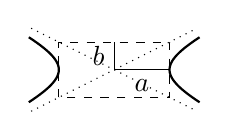
\begin{tikzpicture}[baseline={(0,-5pt)}]
  \def\a{20pt} \def\b{10pt}
  \draw[dashed] (-\a,-\b) rectangle (\a,\b);
  \draw[dotted] (-1.5*\a,-1.5*\b) -- (1.5*\a,1.5*\b);
  \draw[dotted] (-1.5*\a,1.5*\b) -- (1.5*\a,-1.5*\b);
  \draw[thick] plot[domain=-1:1,samples=50] ({\a*cosh(\x)},{\b*sinh(\x)});
  \draw[thick] plot[domain=-1:1,samples=50] ({-\a*cosh(\x)},{\b*sinh(\x)});
  \draw (0,0) -- (\a,0) node[midway,below] {$a$};
  \draw (0,0) -- (0,\b) node[midway,left] {$b$};
\end{tikzpicture}
\end{align*}